\documentclass[border=10pt]{standalone}

\usepackage{tikz}
\usepackage{tikzsymbols}
\usetikzlibrary{calc,patterns,shapes.geometric}

\def\centerarc[#1](#2)(#3:#4:#5){\draw[#1] ($(#2)+({#5*cos(#3)},{#5*sin(#3)})$) arc (#3:#4:#5);}

\begin{document}
	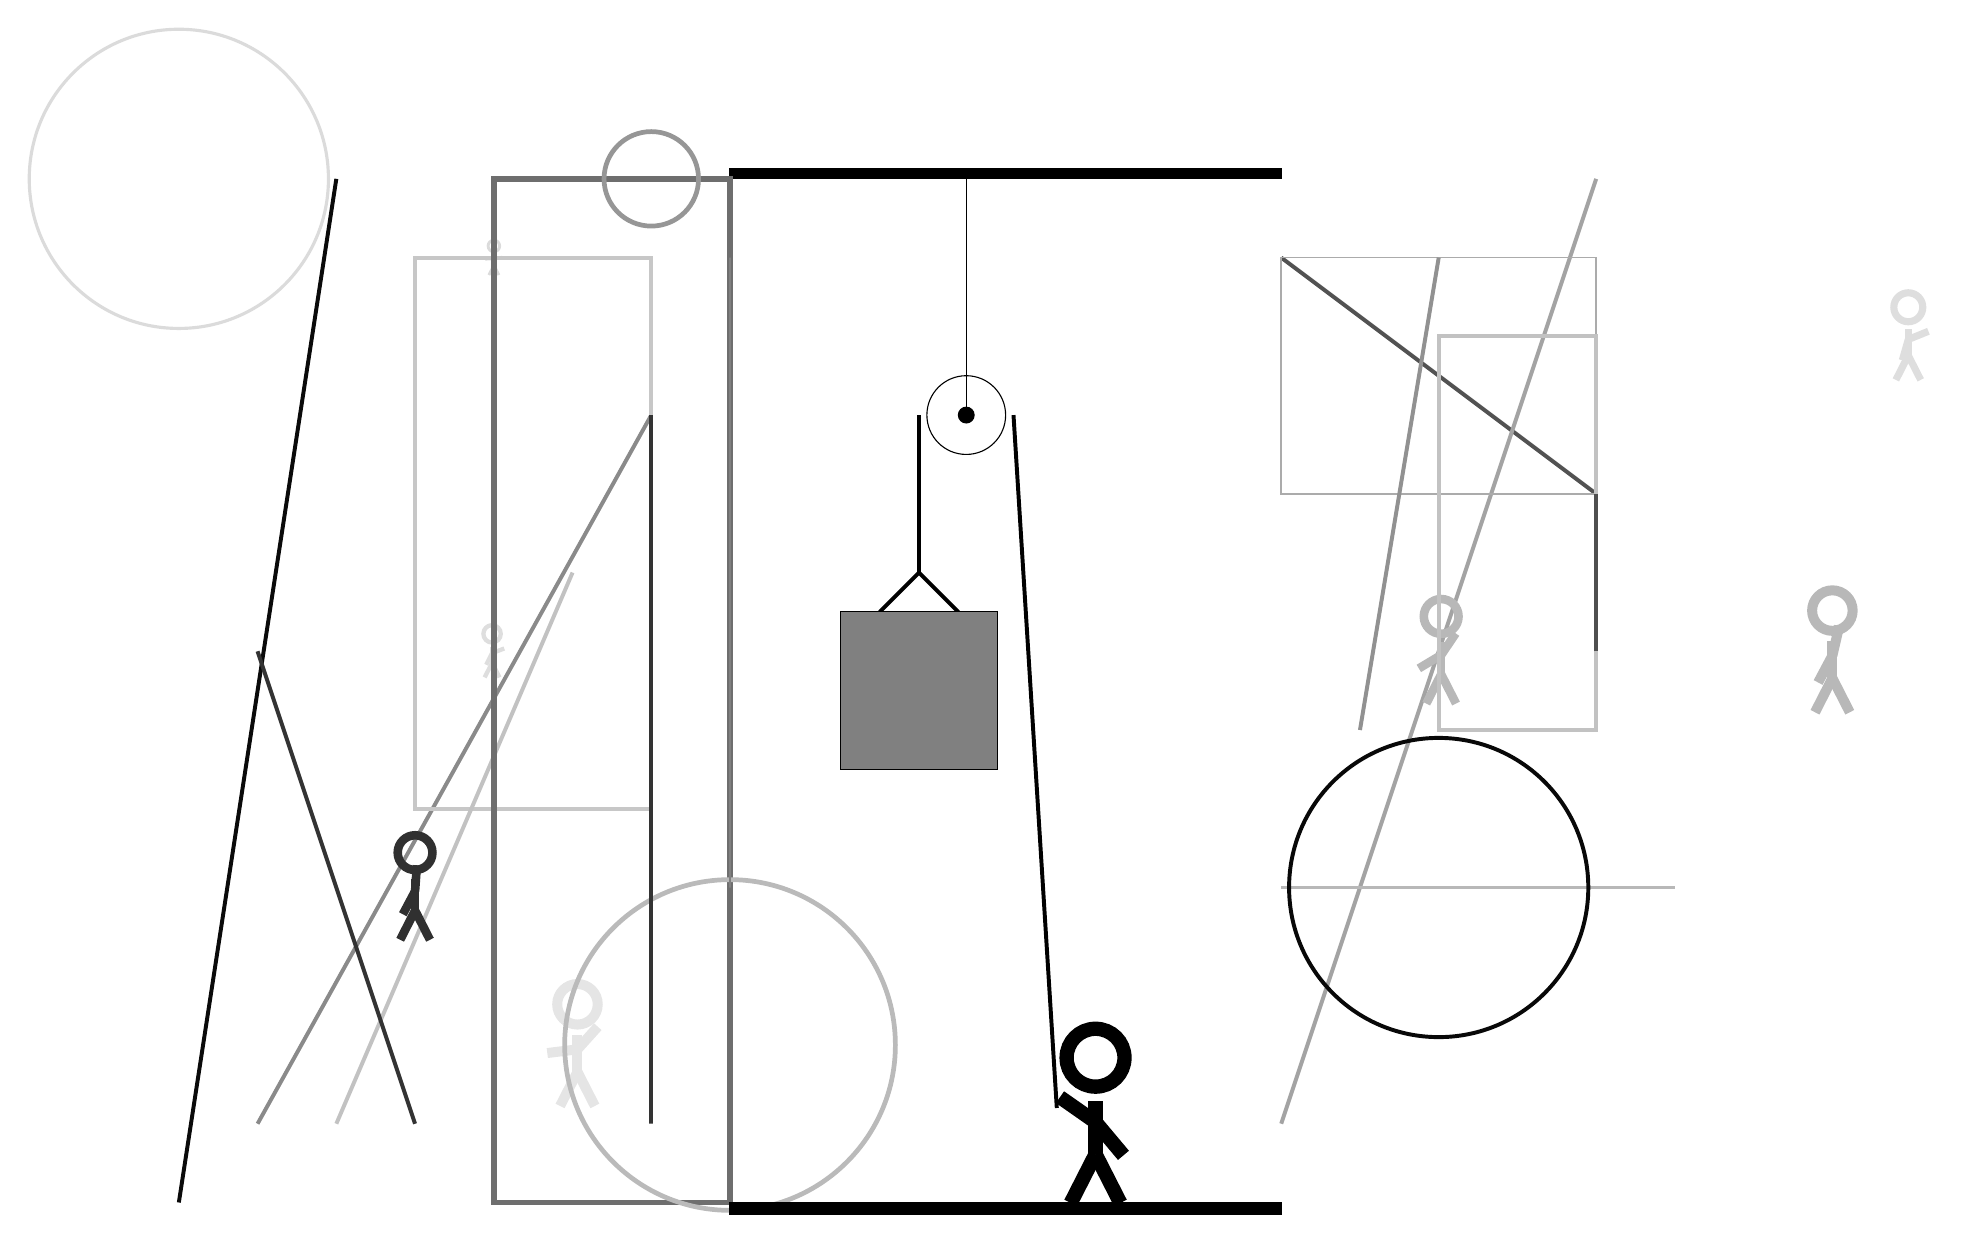
\begin{tikzpicture}
		%%%%% START %%%%%
		
		\draw[fill=black] (-2, 10) rectangle (5, 10.125);
		
		\draw (1, 7) circle (0.5);
		\draw[fill=black] (1, 7) circle (0.1);
		\draw (1, 10) -- (1, 7);
		
		\draw[line width=0.5mm] (-0.1, 4.5) -- (0.4, 5.0) -- (0.9, 4.5);
		\draw[fill=black!50] (-0.6, 4.5) rectangle (1.4, 2.5);
		
		\draw[line width=0.5mm] (0.4, 7) -- (0.4, 5.0);
		\centerarc[line width=0.5mm](1, 7)(0:180:0.6);
		\draw[line width=0.5mm](1.6, 7) -- (2.15, -1.8);
		
		\node at (2.6, -1.9) {\Strichmaxerl[10][-35][-50]};
		
		\draw[line width=0.5mm, color=black!68](5, 9) -- (9, 6);
		
		\draw[line width=0.5mm, color=black!46](-3, 7) -- (-8, -2);
		\draw[line width=0.5mm, color=black!36](5, -2) -- (9, 10);
		\node[line width=0.4mm, color=black!14] at (-5, 9) {\Strichmaxerl[2][2][11]};
		\node[line width=0.2mm, color=black!13] at (-5, 4) {\Strichmaxerl[3][63][21]};
		
		\draw[line width=0.5mm, color=black!22] (-3, 2) rectangle (-6, 9);
		
		\node[line width=0.3mm, color=black!10] at (-4, -1) {\Strichmaxerl[7][7][48]};
		\node[line width=0.3mm, color=black!28] at (7, 4) {\Strichmaxerl[6][31][56]};
		\draw[line width=0.5mm, color=black!28](10, 1) -- (5, 1);
		
		\draw[line width=0.5mm, color=black!24](-4, 5) -- (-7, -2);
		
		\draw[line width=0.7mm, color=black!57] (-2, 10) rectangle (-5, -3);
		\draw [line width=0.5mm, color=black!97](7, 1) circle (1.9);
		\node[line width=0.3mm, color=black!28] at (12, 4) {\Strichmaxerl[7][62][77]};
		
		\draw [line width=0.6mm, color=black!27](-2, -1) circle (2.1);
		\draw [line width=0.6mm, color=black!41](-3, 10) circle (0.6);
		\node[line width=0.2mm, color=black!81] at (-6, 1) {\Strichmaxerl[6][62][86]};
		
		\draw [line width=0.4mm, color=black!14](-9, 10) circle (1.9);
		\draw[line width=0.2mm, color=black!50] (-2, 1) rectangle (-2, 9);
		\draw[line width=0.2mm, color=black!33] (5, 6) rectangle (9, 9);
		\node[line width=0.4mm, color=black!13] at (13, 8) {\Strichmaxerl[5][74][22]};
		\draw[line width=0.5mm, color=black!43](6, 3) -- (7, 9);
		\draw[line width=0.5mm, color=black!80] (-3, -2) rectangle (-3, 7);
		
		\draw[line width=0.5mm, color=black!96](-7, 10) -- (-9, -3);
		\draw[line width=0.5mm, color=black!80](-6, -2) -- (-8, 4);
		\draw[line width=0.5mm, color=black!24] (7, 3) rectangle (9, 8);
		\draw[line width=0.5mm, color=black!69](9, 4) -- (9, 6);
		
		
		\draw[fill=black] (-2, -3) rectangle (5, -3.15);
		
		%%%%% END %%%%%
	\end{tikzpicture}
\end{document}